\documentclass[UTF8,a4paper,zihao=-4]{ctexart}

\usepackage[left=2.35cm,right=2.35cm,top=2.45cm,bottom=2.45cm]{geometry}
\usepackage{amsmath,amssymb}
\usepackage{booktabs,longtable,tabularx,array,multirow}
\usepackage{graphicx,float,caption}
\usepackage{xcolor}
\usepackage{listings}
\usepackage{hyperref,xurl,seqsplit}
\usepackage{fancyhdr}
\usepackage{enumitem}
\usepackage[most]{tcolorbox}
\usepackage{siunitx}
\usepackage{microtype}
\usepackage{tikz}
\usetikzlibrary{arrows.meta,positioning}

\definecolor{navy}{HTML}{274C77}
\definecolor{teal}{HTML}{287271}
\definecolor{coral}{HTML}{B45151}
\definecolor{gold}{HTML}{B8860B}
\definecolor{paper}{HTML}{F6F8FA}
\definecolor{codebg}{HTML}{F3F5F7}
\definecolor{codegreen}{HTML}{1E6B52}
\definecolor{codepurple}{HTML}{6F42C1}

\hypersetup{
  colorlinks=true,
  linkcolor=navy,
  citecolor=teal,
  urlcolor=coral,
  pdftitle={网络安全创新创业实践第五次作业：TenSEAL CKKS 密文卷积},
  pdfauthor={课程作业}
}
\urlstyle{same}

\pagestyle{fancy}
\fancyhf{}
\fancyhead[L]{网络安全创新创业实践}
\fancyhead[R]{第五次作业}
\fancyfoot[C]{\thepage}
\renewcommand{\headrulewidth}{0.4pt}
\setlength{\headheight}{15pt}

\setlength{\parindent}{2em}
\setlength{\parskip}{0.25em}
\setlist{nosep,leftmargin=2.2em}
\captionsetup{font=small,labelfont=bf}
\renewcommand{\arraystretch}{1.22}

\lstdefinestyle{pythonstyle}{
  language=Python,
  backgroundcolor=\color{codebg},
  basicstyle=\ttfamily\scriptsize,
  keywordstyle=\color{codepurple}\bfseries,
  stringstyle=\color{codegreen},
  commentstyle=\color{gray},
  numbers=left,
  numberstyle=\tiny\color{gray},
  numbersep=8pt,
  frame=single,
  rulecolor=\color{gray!35},
  breaklines=true,
  breakatwhitespace=false,
  showstringspaces=false,
  keepspaces=true,
  columns=fullflexible,
  tabsize=4
}
\lstdefinestyle{datastyle}{
  backgroundcolor=\color{codebg},
  basicstyle=\ttfamily\scriptsize,
  frame=single,
  rulecolor=\color{gray!35},
  breaklines=true,
  breakatwhitespace=false,
  columns=fullflexible,
  showstringspaces=false
}

\newtcolorbox{resultbox}[1][]{
  enhanced,
  colback=teal!5,
  colframe=teal!75!black,
  boxrule=0.8pt,
  arc=1.5mm,
  title=#1,
  fonttitle=\bfseries
}
\newtcolorbox{warningbox}[1][]{
  enhanced,
  colback=coral!5,
  colframe=coral!80!black,
  boxrule=0.8pt,
  arc=1.5mm,
  title=#1,
  fonttitle=\bfseries
}

\begin{document}

\begin{titlepage}
  \centering
  \vspace*{1.8cm}
  {\zihao{1}\bfseries 网络安全创新创业实践\par}
  \vspace{0.8cm}
  {\color{navy}\rule{0.78\textwidth}{1.4pt}\par}
  \vspace{1.25cm}
  {\zihao{2}\bfseries 第五次作业\par}
  \vspace{0.45cm}
  {\zihao{3}\bfseries 基于 TenSEAL CKKS 的\par}
  {\zihao{3}\bfseries 单输入单输出密文卷积\par}
  \vspace{1.8cm}
  \begin{tcolorbox}[width=0.76\textwidth,colback=paper,colframe=navy!65,arc=1mm]
    \centering
    \begin{tabular}{rl}
      姓名： & \rule{7cm}{0.4pt}\\[0.7em]
      学号： & \rule{7cm}{0.4pt}\\[0.7em]
      班级： & \rule{7cm}{0.4pt}\\[0.7em]
      完成日期： & 2026年7月24日
    \end{tabular}
  \end{tcolorbox}
  \vfill
  {\large 课程实验报告\par}
  \vspace{0.8cm}
\end{titlepage}

\pagenumbering{Roman}
\begin{abstract}
本作业选择开源全同态加密库 TenSEAL 0.3.16，以 Microsoft SEAL 为后端，完成单输入、单输出的 $4\times4$ 输入与 $3\times3$ 卷积核密文卷积。步长为 1、填充为 0，按 CNN Conv2D 的互相关语义得到 $2\times2$ 输出。客户端使用 CKKS 参数 $N=8192$、系数模数位长链 $[60,40,40,60]$ 和全局缩放因子 $2^{40}$，通过 \texttt{im2col\_encoding} 将四个滑动窗口打包并加密；服务器只持有不含私钥的公开评估上下文，使用 \texttt{conv2d\_im2col} 完成密文与明文卷积核的乘加，客户端最终解密。

明文手算和独立 Python 参考实现均得到
$\left[\begin{smallmatrix}26&31\\46&51\end{smallmatrix}\right]$。对完整流程执行 10 次独立试验，10 个输入密文的 SHA-256 均不同，全部输出满足 $10^{-3}$ 绝对误差阈值；所有试验的最大绝对误差为 $6.882\times10^{-6}$，平均绝对误差为 $5.106\times10^{-6}$。服务器上下文的 \texttt{has\_secret\_key} 和 \texttt{is\_private} 均为 false。中位耗时分别为加密与序列化 \SI{10.402}{ms}、服务器加载/计算/序列化 \SI{14.575}{ms}、客户端加载与解密 \SI{2.328}{ms}。报告给出原始要求、资料学习、算法推导、威胁模型、代码、运行结果、可视化、自动化测试、局限和参考文献。

\noindent\textbf{关键词：}全同态加密；CKKS；TenSEAL；Microsoft SEAL；密文卷积；im2col；SIMD 打包
\end{abstract}

\tableofcontents
\clearpage
\pagenumbering{arabic}

\section{作业原文、任务解释与验收标准}

\subsection{作业原文}

“第五次作业”目录中 \texttt{实验要求.txt} 的原文为：

\begin{quote}
\textbf{作业5：选择任一开源全同态加密库（CPU或GPU均可），使用单输入单输出 $4\times4$ 输入和 $3\times3$ 卷积核（步长1，无填充），实现密文卷积并验证结果正确性。}
\end{quote}

\subsection{严格化解释}

本报告将要求转换为以下可验证条件：

\begin{enumerate}
  \item 开源库必须是真正实现基于格的同态加密，而非自行模拟“加密后计算”；本实验选用 Apache-2.0 许可的 TenSEAL，并固定版本 0.3.16。
  \item “单输入单输出”解释为卷积层输入通道数 $C_{\rm in}=1$、输出通道数 $C_{\rm out}=1$。张量形状为 $[1,1,4,4]$，卷积核形状为 $[1,1,3,3]$。
  \item 步长 $S=1$、填充 $P=0$，故输出高宽必须均为
  \[
    \left\lfloor\frac{4+2P-3}{S}\right\rfloor+1=2.
  \]
  \item 输入必须在服务器计算期间保持密文态；服务器上下文不得含私钥。卷积核是服务器明文模型参数，本实验保护输入隐私，不声称保护模型参数。
  \item 正确性由手工推导、独立明文实现、密文解密结果三方交叉验证。CKKS 是近似方案，因此以预先固定的绝对误差阈值 $10^{-3}$ 判断，而非要求浮点逐位相等。
  \item 保留参数、密钥边界、密文大小、计时、每次试验误差、密文哈希、测试输出和完整代码，保证结果可复核。
\end{enumerate}

\section{参考资料学习与技术选型}

\subsection{课程资料要点}

目录中的《全同态密码算法和应用》从 LWE/RLWE 出发，比较 BFV、BGV、CKKS 和 TFHE，并指出卷积属于线性乘加：可使用 SIMD 打包、Rotation 和明文权重乘法实现。其 $4\times4$ 输入、$3\times3$ 核、步长 1、无填充的示例与本题完全对应，还给出四个有效输出槽和 9 个卷积偏移。资料同时强调 CKKS 的 scale、level、Rescale、KeySwitch 和 Galois Key，以及 TenSEAL 适合快速验证加密张量计算\cite{localfhe}。

《对称密码的软件实现与优化》和《SM3 软件实现》主要讨论 CPU 寄存器、SIMD、指令级并行、缓存、内存访问和不同架构的性能差异\cite{localsymmetric,localsm3}。它们并不直接定义 FHE 卷积，但提供了两条重要工程原则：第一，性能结论必须标注硬件和软件环境；第二，不能只统计抽象运算次数，还应关注大密钥和密文造成的内存流量。本实验因此同时记录计算时间和序列化大小。

\subsection{开源库比较}

\begin{table}[H]
\centering
\caption{候选开源库与本题适配性}
\label{tab:library-choice}
\begin{tabularx}{\textwidth}{>{\raggedright\arraybackslash}p{0.15\textwidth}>{\raggedright\arraybackslash}p{0.22\textwidth}X >{\raggedright\arraybackslash}p{0.14\textwidth}}
\toprule
库 & 主要方案 & 与本题相关特点 & 选择结论\\
\midrule
Microsoft SEAL & BFV、BGV、CKKS & 成熟 C++ 后端，参数检查严格；需要自行完成更多张量封装 & 可行，开发量较大\\
OpenFHE & BGV、BFV、CKKS、FHEW、TFHE & 方案全面，适合深入研究和复杂评测 & 可行，接口较重\\
TenSEAL & BFV、CKKS & 基于 SEAL，直接提供加密向量、\texttt{im2col} 和卷积 API\cite{tenseal,tensealconv} & \textbf{采用}\\
Concrete ML & TFHE & 自动量化与模型转换能力强 & 本题过小，不需完整编译链\\
\bottomrule
\end{tabularx}
\end{table}

CKKS 原论文将加密噪声解释为近似计算误差的一部分，并用 Rescale 管理数值尺度，支持复数/实数向量的批处理\cite{ckks}。本题卷积只含密文与明文权重的线性乘加，乘法深度浅，无需 Bootstrapping；这与 CKKS 和 TenSEAL 的优势吻合。

\section{理论基础与安全边界}

\subsection{RLWE 与 CKKS 近似语义}

CKKS 建立在多项式环
\[
  R_q=\mathbb{Z}_q[X]/(X^N+1)
\]
上的 RLWE 安全结构之上。编码器把槽向量 $\boldsymbol{z}\in\mathbb{C}^{N/2}$ 通过典范嵌入映射到环元素，并乘缩放因子 $\Delta$ 后取整。简化地写，私钥 $s$ 下的二元密文满足
\[
  c_0+c_1s=m+e\pmod q,
\]
其中 $m$ 是编码后的消息，$e$ 是小噪声。解密和解码恢复的是近似值。与 BFV/BGV 的精确整数语义不同，CKKS 的正确性应表述为
\[
  \lVert \operatorname{Decode}(\operatorname{Dec}(ct))-\boldsymbol{z}\rVert_\infty\le\varepsilon.
\]
本实验在运行前固定 $\varepsilon=10^{-3}$，避免观察结果后再放宽阈值。

\subsection{同态线性运算}

卷积核由服务器持有，因而每个权重是明文常量。密文加法和密文乘明文分别为
\[
  (c_0,c_1)+(d_0,d_1)=(c_0+d_0,c_1+d_1),
\]
\[
  p(c_0,c_1)=(pc_0,pc_1).
\]
密文乘明文不会产生 $s^2$ 项，故不需要因该乘法执行重线性化；但 SIMD 槽旋转会改变对应的密钥表示，需要 Galois Key 完成 KeySwitch。TenSEAL 的卷积接口封装了旋转、逐槽明文乘法和累加。

\subsection{威胁模型}

本实验采用诚实但好奇的服务器模型：服务器按协议计算，但可能试图从收到的数据推断用户输入。客户端持有私钥、生成 Galois Key、加密输入并解密结果；服务器只得到公钥、评估密钥、加密输入和明文卷积核。评估密钥允许特定同态变换，但不等价于解密密钥。程序在服务器函数入口检查：
\[
  \texttt{is\_private=False},\qquad \texttt{has\_secret\_key=False}.
\]

\begin{figure}[H]
\centering
\begin{tikzpicture}[
  node distance=1.15cm and 1.35cm,
  box/.style={draw=navy,fill=navy!5,rounded corners=1mm,minimum width=3.4cm,minimum height=1.0cm,align=center},
  server/.style={draw=teal,fill=teal!6,rounded corners=1mm,minimum width=4.1cm,minimum height=1.0cm,align=center},
  arr/.style={-{Latex[length=2.5mm]},thick,draw=gray!75}
]
  \node[box] (keygen) {客户端：CKKS 参数与密钥生成\\保留 secret key};
  \node[box,below=of keygen] (encrypt) {im2col 编码并加密\\序列化输入密文};
  \node[server,right=of encrypt] (eval) {服务器：公开评估上下文\\密文卷积，无法解密};
  \node[box,below=2.2cm of encrypt] (decrypt) {客户端：加载返回密文\\解密并恢复 $2\times2$ 输出};
  \draw[arr] (keygen) -- (encrypt);
  \draw[arr] (encrypt) -- node[above,align=center]{公开上下文+密文\\不含私钥} (eval);
  \draw[arr] (eval) |- node[pos=0.72,above]{输出密文} (decrypt);
\end{tikzpicture}
\caption{客户端与服务器的密钥和数据边界}
\label{fig:threat-model}
\end{figure}

\begin{warningbox}[边界说明]
本实验只保护客户端输入。服务器知道卷积核、参数、输入形状和输出形状，也能观察密文长度与计算时序；未实现模型隐私、访问模式隐藏、主动恶意服务器证明或侧信道防护。实验使用库提供的密码实现，不把自行编写的明文参考函数当作密码组件。
\end{warningbox}

\section{卷积定义、手算与 im2col}

\subsection{CNN Conv2D 语义}

深度学习框架通常把名为 convolution 的算子实现为不翻转卷积核的二维互相关\cite{convguide}。对于本题，输出为
\[
  y_{i,j}=\sum_{u=0}^{2}\sum_{v=0}^{2}x_{i+u,j+v}k_{u,v},
  \qquad i,j\in\{0,1\}.
\]
若使用数学信号处理中“先翻转卷积核”的定义，数值会不同。因此程序和报告均显式声明采用 CNN Conv2D 语义。

实验输入与卷积核为
\[
X=\begin{bmatrix}
1&2&3&4\\
5&6&7&8\\
9&10&11&12\\
13&14&15&16
\end{bmatrix},\qquad
K=\begin{bmatrix}
1&-1&2\\
0&3&-2\\
2&1&-1
\end{bmatrix}.
\]

\subsection{四个输出的独立手算}

\begin{align*}
y_{0,0}={}&1-2+6+0+18-14+18+10-11=26,\\
y_{0,1}={}&2-3+8+0+21-16+20+11-12=31,\\
y_{1,0}={}&5-6+14+0+30-22+26+14-15=46,\\
y_{1,1}={}&6-7+16+0+33-24+28+15-16=51.
\end{align*}
故明文参考输出是
\[
Y=\begin{bmatrix}26&31\\46&51\end{bmatrix}.
\]

\subsection{im2col 变换}

将四个 $3\times3$ 窗口按行展开，得到
\[
W=\begin{bmatrix}
1&2&3&5&6&7&9&10&11\\
2&3&4&6&7&8&10&11&12\\
5&6&7&9&10&11&13&14&15\\
6&7&8&10&11&12&14&15&16
\end{bmatrix},
\]
卷积核向量为
\[
\boldsymbol{k}=[1,-1,2,0,3,-2,2,1,-1]^{\mathsf T}.
\]
因此卷积等价于矩阵向量乘法
\[
W\boldsymbol{k}=[26,31,46,51]^{\mathsf T}.
\]
TenSEAL 的 \texttt{im2col\_encoding} 将四个窗口组织成供旋转与批量内积使用的 CKKS 向量。本次返回的逻辑窗口数为 4，加密向量长度为 64；\texttt{conv2d\_im2col} 一次返回四个逻辑输出槽。

\section{程序设计与实现}

\subsection{代码结构}

\begin{table}[H]
\centering
\caption{作业代码与证据文件}
\label{tab:files}
\begin{tabularx}{\textwidth}{>{\ttfamily\small}p{0.37\textwidth}>{\raggedright\arraybackslash}X}
\toprule
文件 & 职责\\
\midrule
fhe\_convolution.py & 参数检查、明文参考卷积、客户端/服务器上下文分离、加密、密文计算、解密、10 次试验与 JSON 证据\\
test\_fhe\_convolution.py & 手算结果、非法形状、步长、密钥隔离、密文卷积精度和随机化加密测试\\
visualize\_results.py & 从最终 JSON 生成矩阵/误差图和运行验证汇总图\\
requirements.txt & 固定 TenSEAL、Matplotlib 和 NumPy 版本\\
output/experiment\_results.json & 参数、每次密文哈希、误差、计时、大小和最终判定\\
output/figures/ & 报告使用的两张程序生成图片\\
\bottomrule
\end{tabularx}
\end{table}

\subsection{客户端/服务器分离的核心代码}

以下代码片段体现私钥不进入服务器的关键路径：

\begin{lstlisting}[style=pythonstyle]
client_context = create_client_context(parameters)

evaluation_context_bytes = client_context.serialize(
    save_public_key=True,
    save_secret_key=False,
    save_galois_keys=True,
    save_relin_keys=True,
)
server_context = ts.context_from(evaluation_context_bytes)

encrypted_input, windows, _ = client_encrypt_im2col(
    client_context, image
)
encrypted_output = server_encrypted_convolution(
    server_context, encrypted_input, kernel, windows
)
decrypted = client_decrypt_output(
    client_context, encrypted_output, windows
)
\end{lstlisting}

服务器计算函数再次做防御性检查：

\begin{lstlisting}[style=pythonstyle]
if server_context.is_private() or server_context.has_secret_key():
    raise RuntimeError(
        "refusing to evaluate with a secret-bearing server context"
    )
encrypted = ts.ckks_vector_from(server_context, encrypted_input)
result = encrypted.conv2d_im2col(kernel, windows)
return result.serialize()
\end{lstlisting}

这种结构比在同一进程对象上直接“加密、计算、解密”更能表达真实远程推理边界。尽管实验在一台计算机上运行，数据通过序列化字节在两套上下文间传递，服务器对象确实没有私钥。

\section{参数选择与正确性判据}

\subsection{CKKS 参数}

\begin{table}[H]
\centering
\caption{CKKS 参数及理由}
\label{tab:params}
\begin{tabularx}{\textwidth}{p{0.28\textwidth}p{0.25\textwidth}X}
\toprule
参数 & 取值 & 理由\\
\midrule
多项式模数次数 $N$ & 8192 & 提供 $N/2=4096$ 个复数槽，足以容纳本题打包；兼顾演示速度与安全参数\\
系数模数位长链 & $[60,40,40,60]$ & 总位长 200；低于 HE Standard/SEAL 对 $N=8192$、128 bit 目标安全级别常用的 218 bit 上限\cite{hestandard,seal}\\
全局 scale & $2^{40}$ & 提供约 40 bit 小数精度，并与中间 40 bit 素数匹配\\
Galois Key & 生成 & \texttt{conv2d\_im2col} 需要槽旋转\\
Relinearization Key & 序列化保留 & 通用评估上下文保留；本题主路径为密文乘明文，不依赖密文乘密文\\
Bootstrapping & 不使用 & 卷积是浅层线性计算，模数链预算充足\\
\bottomrule
\end{tabularx}
\end{table}

TenSEAL/SEAL 在构造上下文时执行参数合法性检查。这里的“128 bit”是目标经典安全级别，不是说输出有 128 bit 数值精度。参数安全性、数值精度和计算深度是不同概念，不能混为一谈。

\subsection{误差判据}

对第 $t$ 次试验，定义
\[
e_{t,i,j}=\left|\widehat{y}_{t,i,j}-y_{i,j}\right|,
\qquad
E_\infty=\max_{t,i,j}e_{t,i,j}.
\]
通过条件是
\[
E_\infty\le10^{-3},
\]
并且输出形状为 $2\times2$、服务器无私钥、10 次输入密文序列化结果的 SHA-256 全部不同。密文哈希互异只能证明本次观测到加密随机化生效，不构成对随机数生成器熵质量的形式化证明。

\section{运行结果与验证}

\subsection{环境与控制台结果}

实验环境为 Windows 11、Python 3.12.9、TenSEAL 0.3.16，后端为 Microsoft SEAL。执行：

\begin{lstlisting}[style=datastyle]
python fhe_convolution.py --trials 10 \
  --output output/experiment_results.json
\end{lstlisting}

关键输出为：

\begin{lstlisting}[style=datastyle]
TEN SEAL CKKS ENCRYPTED CONVOLUTION
====================================
input shape   : [1, 1, 4, 4]
kernel shape  : [1, 1, 3, 3]
output shape  : [1, 1, 2, 2]
stride/padding: 1/0
plain result  : [[26.0, 31.0], [46.0, 51.0]]
decrypt result: [[26.000003036778416, 31.000004199480824],
                 [46.000006376746114, 51.000006842397156]]
max abs error : 6.881520243e-06
tolerance     : 1.0e-03
trials passed : 10/10
randomized ct : 10/10 unique
server has sk : False
input ct bytes: 334,372
output ct bytes: 235,338
median encrypt: 10.402 ms
median server : 14.575 ms
median decrypt: 2.328 ms
RESULT        : PASS
\end{lstlisting}

\begin{figure}[H]
  \centering
  
\includegraphics[width=\textwidth]{../code/output/figures/runtime_validation.png}
  \caption{程序根据最终 JSON 生成的运行验证汇总图}
  \label{fig:runtime}
\end{figure}

\subsection{数值误差}

最后一次试验的逐槽结果见表~\ref{tab:errors}。10 次试验中的全局最大误差略大于该表最大值，但仍只有 $6.882\times10^{-6}$。

\begin{table}[H]
\centering
\caption{最后一次密文卷积的逐槽误差}
\label{tab:errors}
\begin{tabular}{c c S[table-format=2.0] S[table-format=2.15] S[scientific-notation=true,table-format=1.4e-1]}
\toprule
$i$ & $j$ & {明文参考值} & {CKKS 解密值} & {绝对误差}\\
\midrule
0&0&26&26.000003036778416&3.0368e-6\\
0&1&31&31.000004199480824&4.1995e-6\\
1&0&46&46.000006376746114&6.3767e-6\\
1&1&51&51.000006842397156&6.8424e-6\\
\bottomrule
\end{tabular}
\end{table}

\begin{figure}[H]
  \centering
  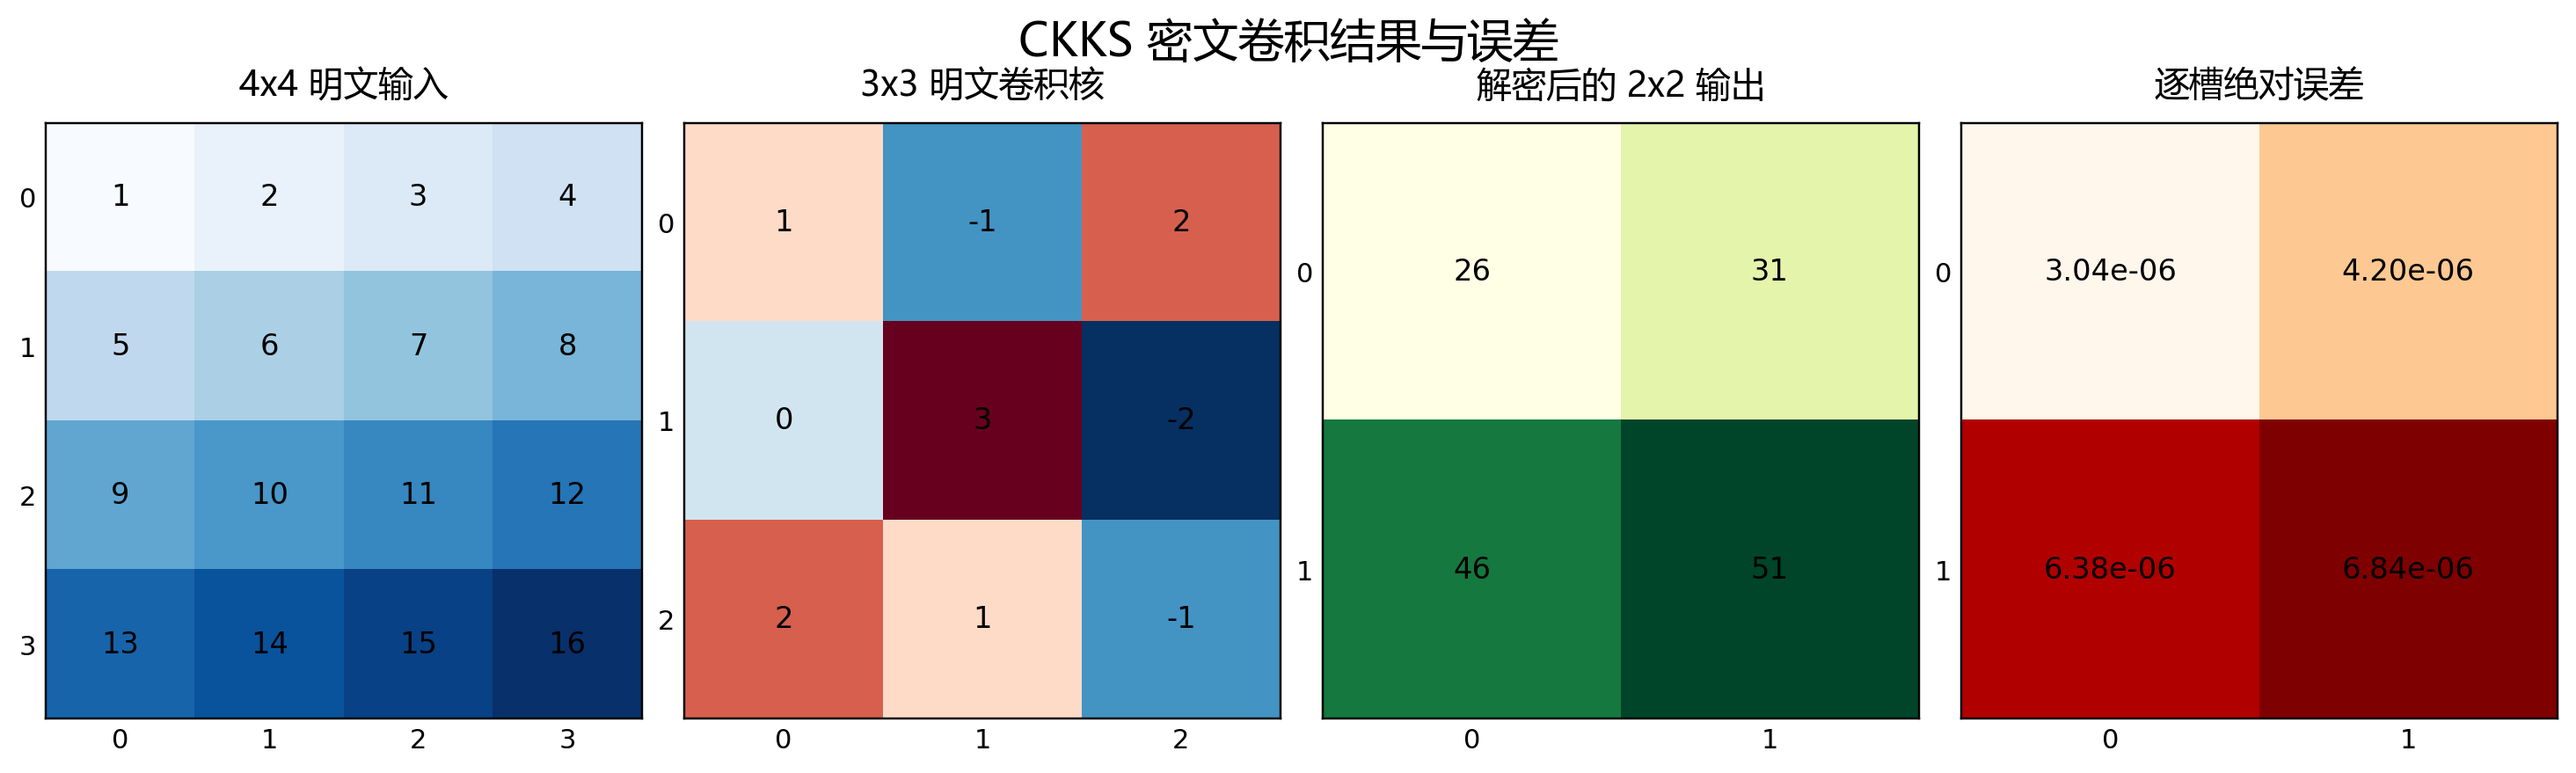
\includegraphics[width=\textwidth]{../code/output/figures/encrypted_convolution_result.png}
  \caption{输入、卷积核、解密输出与逐槽绝对误差}
  \label{fig:matrix-error}
\end{figure}

\begin{resultbox}[正确性结论]
手算、独立明文函数和密文解密的输出形状均为 $2\times2$；明文结果完全一致，10 次密文结果全部满足预先设定的 $10^{-3}$ 误差阈值。$E_\infty=6.882\times10^{-6}$，仅为阈值的约 $0.688\%$。因此在 CKKS 的近似语义下，结果正确。
\end{resultbox}

\subsection{时间与空间开销}

\begin{table}[H]
\centering
\caption{10 次试验的中位耗时与序列化大小}
\label{tab:performance}
\begin{tabularx}{\textwidth}{X r}
\toprule
指标 & 数值\\
\midrule
上下文和密钥初始化 & \SI{1337.975}{ms}\\
客户端 im2col 加密与序列化中位数 & \SI{10.402}{ms}\\
服务器加载、密文卷积与序列化中位数 & \SI{14.575}{ms}\\
客户端加载与解密中位数 & \SI{2.328}{ms}\\
客户端私有上下文序列化 & \num{705215} B\\
服务器公开评估上下文序列化 & \num{35472727} B\\
输入密文序列化 & \num{334372} B\\
输出密文序列化 & \num{235338} B\\
\bottomrule
\end{tabularx}
\end{table}

原始 $4\times4$ 双精度输入仅为 128 B，而打包后输入密文约 334 KB；公开评估上下文约 35.5 MB，主要来自 Galois Keys。这说明 FHE 的主要代价不只在算术，也在密钥和密文数据移动。当前代码为通用性生成完整 Galois Key 集；生产实现可按实际旋转步选择密钥，减少传输和存储。计时仅反映本机、小规模单进程实验，不应外推为通用吞吐量结论。

\section{自动化测试与复现方法}

\subsection{测试结果}

执行 \texttt{python -m unittest -v}，结果为：

\begin{lstlisting}[style=datastyle]
test_ckks_encryption_is_randomized ................. ok
test_encrypted_convolution_matches_reference ....... ok
test_plaintext_reference ........................... ok
test_server_has_no_secret_key ...................... ok
test_shape_and_stride_validation ................... ok
----------------------------------------------------------------------
Ran 5 tests in 1.611s
OK
\end{lstlisting}

测试不仅检查“程序能运行”，还覆盖以下负面条件：$4\times4$ 之外的输入必须拒绝，步长 2 必须拒绝，服务器上下文必须不含私钥，两次相同输入加密的序列化密文必须不同。

\subsection{完整复现命令}

在“第五次作业”目录的 \texttt{code} 子目录中执行：

\begin{lstlisting}[style=datastyle]
python -m pip install -r requirements.txt
python -m py_compile fhe_convolution.py \
  test_fhe_convolution.py visualize_results.py
python -m unittest -v
python fhe_convolution.py --trials 10 \
  --output output/experiment_results.json
python visualize_results.py
\end{lstlisting}

由于 CKKS 加密使用随机数，每次运行的密文哈希、末位近似误差和耗时会变化；明文参考矩阵、输出形状、误差阈值和通过结论应保持不变。JSON 文件保存每次试验的实际值，报告中的数字对应 2026年7月24日的最终采样。

\section{讨论、局限与改进方向}

\subsection{为什么本题不需要 Bootstrapping}

本题只有一层线性卷积，核心是密文乘明文和密文加法。它不像深层 CNN 那样连续消耗大量 level，也没有 ReLU、MaxPool 等比较型非线性。因此使用 Leveled CKKS 的有限模数链即可完成，Bootstrapping 会增加大量不必要开销。

\subsection{实现局限}

\begin{enumerate}
  \item \textbf{近似而非精确：}CKKS 解密值不是逐位精确整数。若业务要求严格整数等式，可改用 BFV/BGV，并重新设计批处理和明文模数。
  \item \textbf{仅保护输入：}卷积核是明文。若要求模型也保密，需要密文乘密文或多方协议，计算深度、密钥管理和开销均会变化。
  \item \textbf{形状固定：}程序有意严格限定题目要求的 $4\times4$、$3\times3$、stride 1、padding 0；这使错误输入无法悄然得到其他输出。
  \item \textbf{评估密钥较大：}当前完整 Galois Key 集导致公开上下文约 35.5 MB。可根据所需 Rotation 精简密钥。
  \item \textbf{性能样本有限：}仅在一台 Windows CPU 上执行 10 次，未固定 CPU 频率、线程绑定或系统负载，计时用于复现当前实验，不是严谨的跨平台基准。
  \item \textbf{未覆盖恶意行为和侧信道：}服务器返回错误密文时客户端只能发现数值异常；未加入可验证计算证明，也未评估缓存、分支、功耗或通信元数据侧信道。
\end{enumerate}

\subsection{可扩展方向}

后续可对比 BFV 精确整数卷积与 CKKS 近似卷积；针对多通道卷积研究通道/空间联合打包；只生成必要旋转的 Galois Keys；增加误差随 scale 和模数链变化的参数扫描；在相同安全级别下比较 CPU、GPU 和 FPGA 的延迟、吞吐与能耗。对于完整 CNN，还需把 BatchNorm 融合到卷积，把 ReLU/MaxPool 替换为 HE 友好近似，并在整张计算图上联合规划 level 和 scale。

\section{结论}

本作业使用真正的开源 FHE 库 TenSEAL 完成了规定的单输入单输出密文卷积。客户端加密 $4\times4$ 输入，服务器在无私钥上下文中对 $3\times3$ 明文卷积核执行 stride 1、padding 0 的密文卷积，客户端解密得到 $2\times2$ 输出。手算和独立明文实现均为 $[[26,31],[46,51]]$；10 次随机化加密全部通过，最大绝对误差 $6.882\times10^{-6}<10^{-3}$，服务器私钥检查为 false。代码、JSON、图片、测试和完整报告共同形成了可运行、可验证、边界陈述准确的交付。

\clearpage
\appendix
\section{交付文件索引}

\begin{longtable}{p{0.50\textwidth}>{\raggedright\arraybackslash}p{0.40\textwidth}}
\toprule
相对路径 & 内容\\
\midrule
\endhead
\path{code/fhe_convolution.py} & 密文卷积主程序和实验驱动\\
\path{code/test_fhe_convolution.py} & 5 项自动化测试\\
\path{code/visualize_results.py} & 两张报告图片的生成程序\\
\path{code/requirements.txt} & 固定依赖版本\\
\path{code/README.md} & 运行说明与安全边界\\
\path{code/output/experiment_results.json} & 10 次试验的完整机器可读证据\\
\path{code/output/figures/encrypted_convolution_result.png} & 矩阵与误差可视化\\
\path{code/output/figures/runtime_validation.png} & 运行验证汇总图\\
\path{report/main.tex} & 本报告 LaTeX 源文件\\
\path{report/main.pdf} & 编译后的最终报告\\
\bottomrule
\end{longtable}

\section{完整源代码}

\subsection{fhe\_convolution.py}
\lstinputlisting[style=pythonstyle]{../code/fhe_convolution.py}

\subsection{test\_fhe\_convolution.py}
\lstinputlisting[style=pythonstyle]{../code/test_fhe_convolution.py}

\subsection{visualize\_results.py}
\lstinputlisting[style=pythonstyle]{../code/visualize_results.py}

\clearpage
\begin{thebibliography}{99}
\raggedright

\bibitem{ckks}
Jung Hee Cheon, Andrey Kim, Miran Kim, Yongsoo Song.
\textit{Homomorphic Encryption for Arithmetic of Approximate Numbers}.
ASIACRYPT 2017; Cryptology ePrint Archive, Paper 2016/421.\\
\url{https://eprint.iacr.org/2016/421}. 访问日期：2026-07-24.

\bibitem{tenseal}
Ayoub Benaissa, Bilal Retiat, Bogdan Cebere, Alaa Eddine Belfedhal.
\textit{TenSEAL: A Library for Encrypted Tensor Operations Using Homomorphic Encryption}.
arXiv:2104.03152, 2021.\\
\url{https://arxiv.org/abs/2104.03152};
\url{https://github.com/OpenMined/TenSEAL}. 访问日期：2026-07-24.

\bibitem{tensealconv}
OpenMined. \textit{TenSEAL Tutorial 4: Encrypted Convolution on MNIST}.\\
\url{https://github.com/OpenMined/TenSEAL/blob/main/tutorials/Tutorial\%204\%20-\%20Encrypted\%20Convolution\%20on\%20MNIST.ipynb}.
访问日期：2026-07-24.

\bibitem{seal}
Microsoft Research. \textit{Microsoft SEAL: An Easy-to-use Open-source Homomorphic Encryption Library}.\\
\url{https://github.com/microsoft/SEAL}. 访问日期：2026-07-24.

\bibitem{hestandard}
HomomorphicEncryption.org. \textit{Homomorphic Encryption Standard, Version 1.1}. 2018.\\
\url{https://homomorphicencryption.org/standard/}. 访问日期：2026-07-24.

\bibitem{convguide}
Vincent Dumoulin, Francesco Visin.
\textit{A Guide to Convolution Arithmetic for Deep Learning}.
arXiv:1603.07285, 2016.\\
\url{https://arxiv.org/abs/1603.07285}. 访问日期：2026-07-24.

\bibitem{localfhe}
课程参考资料：\textit{全同态密码算法和应用}，本地 HTML 课件，2026.

\bibitem{localsymmetric}
付勇. \textit{对称密码的软件实现与优化}. 课程参考资料，2026.

\bibitem{localsm3}
课程参考资料：\textit{SM3 软件实现与优化}. 2026.

\end{thebibliography}

\end{document}
